% =============================================================================
% Module 5: Magnification, Convergence, and Shear
% =============================================================================
% Sources: Narayan & Bartelmann Sec. 3.2, Congdon & Keeton Ch. 2.6 & 4,
%          Saha et al. Sec. 1
% Mathematica: ../Mathematica/05_Magnification_Convergence_Shear/
% =============================================================================

\chapter{Magnification, Convergence, and Shear}
\label{ch:magnification}

\begin{quote}
\textit{Convergence acting alone causes an isotropic focusing of light rays, leading
to an isotropic magnification of a source.  The source is mapped onto an image
with the same shape but larger size.  Shear introduces anisotropy (or
astigmatism) into the lens mapping [\ldots]}
\hfill --- Narayan \& Bartelmann (1997), Sect.~3.2
\end{quote}

\noindent
In Chapter~\ref{ch:lens_equation} we derived the lens equation
$\vecbeta = \vectheta - \vecalpha(\vectheta)$ and used it to find
image positions for a point mass lens.  We also previewed the
magnification formula for the point mass case.  Now we develop the
\textit{general} formalism that describes how lensing distorts images:
their size, shape, and brightness relative to the unlensed source.

The key players are:
\begin{itemize}[nosep]
    \item The \textbf{lensing potential} $\psiL(\vectheta)$, from
          which the deflection angle derives as a gradient.
    \item The \textbf{convergence} $\kappab(\vectheta)$, the
          dimensionless surface mass density, which causes isotropic
          focusing.
    \item The \textbf{shear} $\gammaL(\vectheta)$, a spin-2 field
          that causes anisotropic stretching.
    \item The \textbf{Jacobian matrix} $\Amat$, which encodes
          all local lensing distortions.
    \item The \textbf{magnification} $\mu$, the ratio of image
          area to source area.
\end{itemize}

\medskip
\noindent
\textbf{Companion Mathematica files:}
\begin{itemize}[nosep]
    \item \mathlink{05_Magnification_Convergence_Shear/lensing_potential.wl}{lensing\_potential.wl}
          --- symbolic derivation of $\psiL$, convergence, shear,
          Jacobian, and magnification for the point mass lens;
          verification of the 2D Poisson equation; publication-quality
          figure generation
    \item \mathlink{05_Magnification_Convergence_Shear/convergence_shear_demo.nb}{convergence\_shear\_demo.nb}
          --- interactive notebook: Manipulate for convergence and
          shear effects on circular sources, magnification map for
          point mass lens
\end{itemize}


% =====================================================================
\section{Introduction: From Image Positions to Image Properties}
\label{sec:mag_intro}

The lens equation tells us \textit{where} images form.  But
observations reveal much more than positions: lensed images are
\textit{stretched}, \textit{magnified}, and sometimes
\textit{mirror-reflected} relative to the unlensed source.  Giant arcs
in galaxy clusters are dramatic examples --- background galaxies
stretched into elongated curves by the cluster's gravity.

To describe these distortions quantitatively, we need to understand the
\textit{local} properties of the lens mapping
$\vecbeta(\vectheta)$.  Since the lens mapping is a smooth function
(except at isolated singularities), its local behavior is captured by
its \textbf{Jacobian matrix} --- the matrix of first partial
derivatives.  This matrix encodes all information about magnification,
stretching, and parity of each image.

We begin by introducing the \textbf{effective lensing potential}
$\psiL(\vectheta)$, a scalar field from which the deflection angle
can be derived as a gradient.  This potential provides a unified
framework: its first derivatives give the deflection, and its second
derivatives give the convergence and shear.


% =====================================================================
\section{The Effective Lensing Potential}
\label{sec:lensing_potential}

In Chapter~\ref{ch:lens_equation} (eq.~\ref{eq:alpha_angular}) we
expressed the reduced deflection angle as an integral over the
convergence.  Remarkably, this deflection can be written as the
gradient of a scalar potential.

\begin{definition}
The \textbf{effective lensing potential} (or simply the lensing
potential) is defined as
(Narayan \& Bartelmann eq.~51; Congdon \& Keeton eq.~4.14):
\begin{equation}
    \boxed{
    \psiL(\vectheta) = \frac{1}{\pi}
    \int \kappab(\vectheta')\,
    \ln|\vectheta - \vectheta'|\, d^2\theta'
    }
    \label{eq:lensing_potential}
\end{equation}
where $\kappab(\vectheta') = \Sigma(\Dd\,\vectheta')/\Sigmacr$ is
the convergence (eq.~\ref{eq:convergence_def}) and the integral
extends over the entire lens plane.
\end{definition}

This is the two-dimensional analog of the Newtonian gravitational
potential: just as the three-dimensional gravitational potential
$\Phi(\mathbf{r}) = -\Gnewton \int \rho(\mathbf{r}')/|\mathbf{r} -
\mathbf{r}'|\, d^3r'$ satisfies Poisson's equation
$\nabla^2\Phi = 4\pi\Gnewton\rho$, the lensing potential satisfies
the two-dimensional Poisson equation.

\begin{remark}
The lensing potential $\psiL$ is dimensionless when $\vectheta$ is
measured in radians.  It is related to the physical (Shapiro) time
delay through the Fermat potential, which we will encounter in
Module~6.
\end{remark}
\begin{annotation}[What in $\psiL$ is physical?]
Only its second derivatives are directly observable. Adding a constant to $\psiL$
changes nothing. Adding a linear term $\mathbf{a}\cdot\vectheta$ shifts every
deflection by the constant vector $\mathbf{a}$, and therefore every source position by
$-\mathbf{a}$. Since the unlensed source position is never observed, this is
unobservable too, and the Hessian, which is all that enters $\kappab$, $\gammaL$ and
$\mu$, is unchanged. Note also that the logarithmic kernel means $\psiL$ of a
finite mass does \emph{not} vanish at infinity. It grows like
$\ln|\vectheta|$, as the point-mass example $\psiL = \thetaE^2\ln|\vectheta|$
below shows. Do not try to impose $\psiL \to 0$ as a boundary condition.
\end{annotation}

\subsection{Key Properties of the Lensing Potential}

The lensing potential has two crucial properties:

\paragraph{(1) Its gradient gives the deflection angle.}
Taking the gradient of eq.~\eqref{eq:lensing_potential}:
\begin{equation}
    \boxed{
    \vecalpha(\vectheta) = \nabla_\theta\, \psiL(\vectheta)
    }
    \label{eq:alpha_grad_psi}
\end{equation}
where $\nabla_\theta = (\partial/\partial\theta_1,\,
\partial/\partial\theta_2)$ is the two-dimensional gradient with
respect to the angular coordinates.  This can be verified by
differentiating eq.~\eqref{eq:lensing_potential} under the integral
sign and using $\nabla_\theta \ln|\vectheta - \vectheta'| =
(\vectheta - \vectheta')/|\vectheta - \vectheta'|^2$.
\begin{derivation}[Gradient of the potential, step by step]
Write $\ln|\vectheta - \vectheta'| = \tfrac12\ln[(\theta_1 - \theta_1')^2 + (\theta_2 - \theta_2')^2]$.
The chain rule gives
$\partial_{\theta_1}\ln|\vectheta - \vectheta'| = (\theta_1 - \theta_1')/|\vectheta - \vectheta'|^2$,
and likewise for $\theta_2$. The gradient acts on $\vectheta$ only, not on the
integration variable $\vectheta'$, so it passes through the integral:
\begin{equation*}
    \nabla_\theta\psiL = \frac{1}{\pi}\int\kappab(\vectheta')\,
    \frac{\vectheta - \vectheta'}{|\vectheta - \vectheta'|^2}\,d^2\theta' .
\end{equation*}
This is the deflection integral eq.~\eqref{eq:alpha_angular} rewritten with
$\Sigma/\Sigmacr = \kappab$, because its prefactor
$(\Dds/\Ds)(4\Gnewton/\speedoflight^2)\Dd$ equals $1/(\pi\Sigmacr)$. Moving the
derivative inside the integral is legitimate: the kernel diverges only as
$1/|\vectheta - \vectheta'|$, which is integrable in two dimensions.
\end{derivation}

\paragraph{(2) Its Laplacian gives twice the convergence (2D Poisson equation).}
\begin{equation}
    \boxed{
    \nabla^2_\theta\, \psiL(\vectheta) = 2\,\kappab(\vectheta)
    }
    \label{eq:poisson_2d}
\end{equation}
The identity rests on the Green's function of the two-dimensional
Laplacian,
\begin{equation}
    \nabla^2_\theta \ln|\vectheta - \vectheta'|
    \;=\; 2\pi\,\delta^{(2)}(\vectheta - \vectheta') \,,
    \label{eq:green_2d}
\end{equation}
which we prove in two steps.

\textit{Step 1: $\nabla^2 \ln r = 0$ for $r \neq 0$.}
In polar coordinates centered at $\vectheta'$, let $r = |\vectheta -
\vectheta'|$ and write $\nabla^2 = (1/r)\partial_r(r\,\partial_r) +
(1/r^2)\partial_\phi^2$.  Then
$\partial_r(\ln r) = 1/r$ and
$\nabla^2(\ln r) = (1/r)\partial_r(r\cdot 1/r) = (1/r)\partial_r(1)
= 0$ for $r > 0$.

\textit{Step 2: the integrated strength is $2\pi$.}
For any disk $D_a$ of radius $a$ centered at $\vectheta'$, the
divergence theorem gives
\begin{equation*}
    \int_{D_a}\nabla^2 \ln r\,d^2\theta
    \;=\; \oint_{\partial D_a} \nabla(\ln r)\cdot\hat{n}\,d\ell
    \;=\; \oint_{r=a}\!\!\frac{1}{r}\Bigg|_{r=a}\!a\,d\phi
    \;=\; 2\pi.
\end{equation*}
Combined with step 1, $\nabla^2(\ln r)$ is a distribution supported
at the origin with total weight $2\pi$, i.e.\
eq.~\eqref{eq:green_2d}.

Differentiating eq.~\eqref{eq:lensing_potential} under the integral
sign and substituting eq.~\eqref{eq:green_2d}:
\begin{equation}
    \nabla^2_\theta\, \psiL
    \;=\; \frac{1}{\pi}\!\int \kappab(\vectheta')\,
        2\pi\,\delta^{(2)}(\vectheta - \vectheta')\,d^2\theta'
    \;=\; 2\,\kappab(\vectheta) \,.
    \label{eq:poisson_derivation}
\end{equation}
Equivalently, one can bypass eq.~\eqref{eq:green_2d} entirely using
$\vecalpha = \nabla\psiL$ (eq.~\ref{eq:alpha_grad_psi}) and
$\kappab = \frac{1}{2}\nabla\cdot\vecalpha$ (Narayan \& Bartelmann
eq.~56; Congdon \& Keeton eq.~4.22):
$\frac{1}{2}\nabla^2\psiL = \frac{1}{2}\nabla\cdot(\nabla\psiL) =
\frac{1}{2}\nabla\cdot\vecalpha = \kappab$.
Both routes are verified symbolically in
\mathlink{05_Magnification_Convergence_Shear/lensing_potential.wl}{lensing\_potential.wl}
(direct convolution for the point-mass and uniform-disk convergence).
\begin{annotation}[A smooth picture of the delta function]
Step~2 can be made concrete. The smoothed logarithm
$\tfrac12\ln(|\vectheta|^2 + \epsilon^2)$ has Laplacian
$2\epsilon^2/(|\vectheta|^2 + \epsilon^2)^2$. This is a bump of height
$2/\epsilon^2$ and width $\sim\epsilon$ whose integral over the plane is
$2\pi$ for \emph{every} $\epsilon$. As $\epsilon \to 0$ it becomes
$2\pi\,\delta^{(2)}(\vectheta)$. The factor 2 in $\nabla^2\psiL = 2\kappab$ is
this $2\pi$ divided by the $\pi$ in the definition~\eqref{eq:lensing_potential}.
The same identity also follows from the three-dimensional Poisson equation
integrated along the line of sight (Narayan \& Bartelmann eq.~50).
\end{annotation}
\begin{bridge}[Multipoles through the Poisson equation]
Chapter~\ref{ch:multipoles} perturbs a lens by angular multipoles. Each is
most easily written as a potential $\psiL = \theta\,f(\phi)$, and the
corresponding convergence follows from eq.~\eqref{eq:poisson_2d} in polar form,
$\nabla^2 = \theta^{-1}\partial_\theta(\theta\,\partial_\theta) + \theta^{-2}\partial_\phi^2$:
\begin{equation*}
    \kappab = \frac{f(\phi) + f''(\phi)}{2\theta},
    \qquad
    f = \cos m\phi \;\Rightarrow\; \kappab = \frac{(1 - m^2)\cos m\phi}{2\theta}.
\end{equation*}
The $m = 1$ term carries no mass at all: $\theta\cos\phi = \theta_1$ is a
linear potential, a constant deflection that only shifts the unobservable
source position. For $m = 2$ the factor $1 - m^2 = -3$ means that, relative to the
monopole, the $\cos 2\phi$ modulation is three times stronger in $\kappab$
than in $\psiL/\theta$. Adding $\epsilon\,\theta\cos2\phi$ to an
isothermal $\psiL = \thetaE\theta$ makes the isodensity contours about three
times as elongated as the isopotentials, along the same axis. Forgetting the
factor $(1 - m^2)$ when moving between potential and density multipoles is a
common error.
\end{bridge}


% =====================================================================
\section{Convergence}
\label{sec:convergence}

The convergence was already introduced in
Chapter~\ref{ch:lens_equation} (eq.~\ref{eq:convergence_def}):

\begin{equation}
    \kappab(\vectheta) = \frac{\Sigma(\Dd\,\vectheta)}{\Sigmacr}
    \label{eq:kappa_def_review}
\end{equation}

It is the \textbf{dimensionless surface mass density} --- the ratio of
the actual surface mass density to the critical value.  We now explore
its role in image distortion.

\subsection{Physical Meaning}

The convergence measures the \textit{isotropic focusing} caused by
the lens:
\begin{itemize}
    \item A region with $\kappab > 0$ acts as a converging lens,
          focusing light rays and magnifying images isotropically
          (without changing their shape).
    \item $\kappab = 1$ means $\Sigma = \Sigmacr$: this is the
          threshold for strong lensing.  Regions where $\kappab \geq 1$
          are \textbf{supercritical} and can produce multiple images.
    \item For an \textbf{axisymmetric} lens, $\kappab < 1$ everywhere
          means the lens is subcritical: it can still distort images
          (via shear), but it cannot produce multiple images.  (For a
          non-axisymmetric lens, $\kappab > 1$ somewhere is sufficient
          but not necessary: shear can produce multiple images even
          with $\kappab < 1$ everywhere; Congdon \& Keeton Sec.~2.5.)
\end{itemize}

\subsection{Convergence from the Lensing Potential}

From the 2D Poisson equation~\eqref{eq:poisson_2d}:
\begin{equation}
    \kappab(\vectheta) = \frac{1}{2}\,\nabla^2_\theta\, \psiL
    = \frac{1}{2}\left(
    \frac{\partial^2 \psiL}{\partial\theta_1^2}
    + \frac{\partial^2 \psiL}{\partial\theta_2^2}\right) .
    \label{eq:kappa_from_psi}
\end{equation}
Thus the convergence is the \textit{trace} of the Hessian of the
lensing potential (up to a factor of $1/2$).


% =====================================================================
\section{Shear}
\label{sec:shear}

The shear describes the \textit{anisotropic distortion} of images ---
the stretching in one direction and compression in the perpendicular
direction.

The specific combinations that define $\gamma_1$ and $\gamma_2$ are
forced by a clean geometric argument.  The Hessian of the lensing
potential,
\begin{equation*}
    H_{ij} \;\equiv\; \frac{\partial^2 \psiL}{\partial\theta_i\,\partial\theta_j} \,,
\end{equation*}
is a $2{\times}2$ real symmetric matrix --- three independent
components.  Every such matrix decomposes uniquely into a trace piece
(proportional to the identity) plus a traceless symmetric piece:
\begin{equation}
    H \;=\; \frac{\operatorname{tr}H}{2}\,\mathbb{I} + H^{\mathrm{TF}},
    \qquad
    H^{\mathrm{TF}} = \begin{pmatrix}
        \tfrac{1}{2}(H_{11}-H_{22}) & H_{12} \\
        H_{12} & -\tfrac{1}{2}(H_{11}-H_{22})
    \end{pmatrix}.
    \label{eq:hessian_decomp}
\end{equation}
The trace part is the isotropic convergence
$\tfrac{1}{2}\operatorname{tr}H = \kappab$
(eq.~\ref{eq:kappa_from_psi}); the traceless part is the shear.
Its two independent entries are named
\begin{equation}
    \boxed{
    \gamma_1(\vectheta) = \frac{1}{2}\!\left(
    \frac{\partial^2 \psiL}{\partial\theta_1^2}
    - \frac{\partial^2 \psiL}{\partial\theta_2^2}\right) ,
    \qquad
    \gamma_2(\vectheta)
    = \frac{\partial^2 \psiL}{\partial\theta_1\,\partial\theta_2} \,,}
    \label{eq:shear_components}
\end{equation}
so that the Hessian itself reads
$H = \bigl((\kappab + \gamma_1)\;\,\gamma_2;\,\gamma_2\;\,(\kappab -
\gamma_1)\bigr)$.  Under a rotation of the $\vectheta$-axes by angle
$\phi$, $H^{\mathrm{TF}}$ transforms as a rank-2 symmetric tensor
whose traceless part carries \emph{two} powers of $e^{\pm i\phi}$.
Forming the complex shear $\gamma \equiv \gamma_1 + i\gamma_2$,
\begin{equation}
    \gamma \;\longrightarrow\; e^{-2i\phi}\,\gamma \,,
    \label{eq:shear_spin2}
\end{equation}
which is the spin-2 transformation law --- the reason the shear has a
$180^\circ$ (not $360^\circ$) rotational symmetry.  The decomposition
\eqref{eq:hessian_decomp} and the transformation law
\eqref{eq:shear_spin2} are verified symbolically in
\texttt{lensing\_potential.wl}.
\begin{derivation}[The spin-2 law, written out]
Rotate the coordinate axes by $\phi$. The new basis vectors are the columns of
$R = \bigl(\begin{smallmatrix}\cos\phi & -\sin\phi\\ \sin\phi & \cos\phi\end{smallmatrix}\bigr)$,
and a second-rank tensor transforms as $H' = R^{\mathsf T}HR$. Using
$H = \bigl(\begin{smallmatrix}\kappab+\gamma_1 & \gamma_2\\ \gamma_2 & \kappab-\gamma_1\end{smallmatrix}\bigr)$
and the double-angle identities
$\cos^2\phi - \sin^2\phi = \cos2\phi$ and $2\sin\phi\cos\phi = \sin2\phi$:
\begin{align*}
    \kappab' &= \tfrac12\operatorname{tr}H' = \tfrac12\operatorname{tr}H = \kappab
       && \text{(trace is invariant)},\\
    \gamma_1' &= \tfrac12(H'_{11} - H'_{22}) = \gamma_1\cos2\phi + \gamma_2\sin2\phi,\\
    \gamma_2' &= H'_{12} = -\gamma_1\sin2\phi + \gamma_2\cos2\phi .
\end{align*}
Hence $\gamma_1' + i\gamma_2' = (\cos2\phi - i\sin2\phi)(\gamma_1 + i\gamma_2)
= e^{-2i\phi}\gamma$. The angle appears doubled because each of the two
indices of $H$ contributes one factor of $R$.
\end{derivation}

The shear magnitude and the complex shear are:
\begin{equation}
    |\gammaL| = \sqrt{\gamma_1^2 + \gamma_2^2} \,,
    \qquad
    \gammaL = \gamma_1 + i\,\gamma_2 = |\gammaL|\, e^{2i\phi_\gamma}
    \label{eq:shear_magnitude}
\end{equation}
where $\phi_\gamma$ is the orientation angle of the shear.
\begin{annotation}[Shear is a trace-free tensor, not a vector]
Three consequences of spin~2 trip up students. (i) $\gamma \to -\gamma$ is
\emph{not} a reversal of direction: it rotates the stretch axis by
$90^\circ$. (ii) The orientation is
$\phi_\gamma = \tfrac12\operatorname{atan2}(\gamma_2, \gamma_1)$, the
two-argument arctangent. The one-argument
$\tfrac12\arctan(\gamma_2/\gamma_1)$ is off by $90^\circ$ whenever
$\gamma_1 < 0$. For example, $(\gamma_1, \gamma_2) = (-0.1, 0.1)$ has its stretch
axis at $67.5^\circ$, not $-22.5^\circ$. (iii) Shears from different
deflectors add as \emph{tensors}, i.e.\ as the complex numbers
$\gamma_1 + i\gamma_2$, not as magnitudes.
\end{annotation}

\subsection{Physical Meaning}

The shear is a \textbf{spin-2 field}: it is invariant under rotations
by $180°$ (not $360°$), reflecting the fact that an ellipse looks
the same after a half-turn.  The two components have specific geometric
meanings:
\begin{itemize}
    \item $\gamma_1 > 0$: stretching along the $\theta_1$-axis,
          compression along $\theta_2$.
    \item $\gamma_1 < 0$: stretching along the $\theta_2$-axis,
          compression along $\theta_1$.
    \item $\gamma_2 > 0$: stretching along the direction at $45°$
          to the $\theta_1$-axis.
    \item $\gamma_2 < 0$: stretching along the direction at $135°$
          to the $\theta_1$-axis.
\end{itemize}

\begin{remark}
The convergence and shear together account for all four independent
second derivatives of the lensing potential (the Hessian is a
symmetric $2 \times 2$ matrix with three independent components;
$\kappab$ captures the trace, and $\gamma_1$, $\gamma_2$ capture
the traceless part):
\begin{equation}
    \frac{\partial^2 \psiL}{\partial\theta_i\,\partial\theta_j}
    = \begin{pmatrix}
    \kappab + \gamma_1 & \gamma_2 \\
    \gamma_2 & \kappab - \gamma_1
    \end{pmatrix} .
    \label{eq:hessian_decomposition}
\end{equation}
\end{remark}


% =====================================================================
\section{The Jacobian Matrix (Inverse Magnification Tensor)}
\label{sec:jacobian}

The lens equation $\vecbeta = \vectheta - \vecalpha(\vectheta)$
defines a mapping from the image plane to the source plane.  The
local properties of this mapping are encoded in its
\textbf{Jacobian matrix}:
\begin{equation}
    \Amat_{ij} = \frac{\partial \beta_i}{\partial \theta_j}
    = \delta_{ij} - \frac{\partial \alpha_i}{\partial \theta_j}
    = \delta_{ij}
    - \frac{\partial^2 \psiL}{\partial\theta_i\,\partial\theta_j}
    \label{eq:jacobian_def}
\end{equation}
where in the last step we used
$\alpha_i = \partial\psiL/\partial\theta_i$
(eq.~\ref{eq:alpha_grad_psi}).
\begin{derivation}[Index form, and why $\Amat$ is symmetric]
Differentiate $\beta_i = \theta_i - \alpha_i(\vectheta)$ with respect to
$\theta_j$: $\partial\theta_i/\partial\theta_j = \delta_{ij}$ (the coordinates
are independent), and
$\partial\alpha_i/\partial\theta_j = \partial_j\partial_i\psiL$. Because mixed
partial derivatives commute ($\psiL$ is smooth away from point masses),
$\Amat_{12} = \Amat_{21}$: the single-plane Jacobian is \emph{symmetric}. This
is a direct consequence of $\vecalpha$ being a gradient, i.e.\ curl-free.
\end{derivation}
\begin{bridge}[The Jacobian with two lens planes is not symmetric]
With two deflectors the ray hits the second plane at a position that already depends
on the first deflection, so the chain rule gives (schematically)
$\Amat = \mathbf{I} - H_1 - H_2(\mathbf{I} - b\,H_1)$, where $b$ is a
distance factor. The product $H_2H_1$ of two symmetric matrices is in general
not symmetric. The multi-plane Jacobian therefore acquires an antisymmetric
(rotation) part and can be decomposed into a rotation times a symmetric matrix
(Schneider, Ehlers \& Falco Sec.~9.1). Chapter~\ref{ch:multiplane_dspl} uses
this structure. Everything in the present chapter that assumes $\Amat$ is
symmetric (real eigenvalues, orthogonal principal axes, $\kappab$ and
$\gammaL$ as its only content) must be revisited there.
\end{bridge}

Using the decomposition of the Hessian into convergence and shear
(eq.~\ref{eq:hessian_decomposition}), the Jacobian takes the elegant
form (Narayan \& Bartelmann eq.~58; Congdon \& Keeton eq.~4.51):
\begin{equation}
    \boxed{
    \Amat = \begin{pmatrix}
    1 - \kappab - \gamma_1 & -\gamma_2 \\
    -\gamma_2 & 1 - \kappab + \gamma_1
    \end{pmatrix}
    }
    \label{eq:jacobian_matrix}
\end{equation}
\begin{annotation}[Notation in the textbooks]
Narayan \& Bartelmann eq.~58 is identical to eq.~\eqref{eq:jacobian_matrix}.
Congdon \& Keeton use the opposite naming: their $A^{-1}$ (C\&K eq.~4.51) is
\emph{our} $\Amat$, their $A$ (``amplification tensor'', eq.~4.53) is our
$\Mmat$, and they write $\gamma_+, \gamma_\times$ for our $\gamma_1, \gamma_2$
(eq.~4.52). Check which convention a paper uses before copying a sign or an
inverse.
\end{annotation}

\begin{remark}
The matrix $\Amat$ is sometimes called the \textbf{inverse
magnification tensor} because its inverse $\Amat^{-1}$ gives the
magnification tensor $\Mmat$:
\begin{equation}
    \Mmat = \Amat^{-1}
    = \frac{\partial\vectheta}{\partial\vecbeta} \,.
    \label{eq:magnification_tensor}
\end{equation}
$\Mmat$ maps source-plane displacements to image-plane displacements.
\end{remark}

\subsection{Decomposition of the Jacobian}

The Jacobian can be decomposed into a convergence (isotropic) part
and a shear (anisotropic) part:
\begin{equation}
    \Amat = (1 - \kappab)\,
    \begin{pmatrix} 1 & 0 \\ 0 & 1 \end{pmatrix}
    - \begin{pmatrix}
    \gamma_1 & \gamma_2 \\
    \gamma_2 & -\gamma_1
    \end{pmatrix}
    \label{eq:jacobian_decomposition}
\end{equation}

The first term is proportional to the identity matrix and represents
isotropic focusing (convergence).  The second term is a traceless,
symmetric matrix (the shear matrix) that represents anisotropic
distortion.

\subsection{Eigenvalues of the Jacobian}

The eigenvalues of $\Amat$ are
(Congdon \& Keeton eq.~4.54):
\begin{equation}
    \lambda_\pm = 1 - \kappab \pm |\gammaL|
    = (1 - \kappab) \pm \sqrt{\gamma_1^2 + \gamma_2^2} \,.
    \label{eq:eigenvalues}
\end{equation}
These eigenvalues give the inverse magnification along the two
principal axes of the distortion.  The corresponding eigenvectors
define the directions of maximum and minimum stretching.
\begin{derivation}[Eigenvalues and eigenvectors of $\Amat$]
\emph{Eigenvalues.} The characteristic polynomial is
\begin{equation*}
    \det(\Amat - \lambda\mathbf{I})
    = (1 - \kappab - \lambda - \gamma_1)(1 - \kappab - \lambda + \gamma_1) - \gamma_2^2
    = (1 - \kappab - \lambda)^2 - |\gammaL|^2 ,
\end{equation*}
using $(x - \gamma_1)(x + \gamma_1) = x^2 - \gamma_1^2$. Setting it to zero
gives $1 - \kappab - \lambda = \mp|\gammaL|$, i.e.\ $\lambda_\pm = 1 - \kappab \pm |\gammaL|$
(Congdon \& Keeton eq.~4.54).

\emph{Eigenvectors.} Write $\gamma_1 = |\gammaL|\cos2\phi_\gamma$ and
$\gamma_2 = |\gammaL|\sin2\phi_\gamma$, and try $\mathbf{e} = (\cos\phi_\gamma, \sin\phi_\gamma)$.
The first component of $\Amat\mathbf{e}$ is
$(1-\kappab)\cos\phi_\gamma - |\gammaL|(\cos2\phi_\gamma\cos\phi_\gamma + \sin2\phi_\gamma\sin\phi_\gamma)
= (1 - \kappab - |\gammaL|)\cos\phi_\gamma$, by
$\cos(a - b) = \cos a\cos b + \sin a\sin b$; the second component works the
same way with $\sin(a - b)$. So $\Amat\mathbf{e} = \lambda_-\mathbf{e}$, and
the perpendicular vector $(-\sin\phi_\gamma, \cos\phi_\gamma)$ belongs to
$\lambda_+$. Because an image's extent along an eigenvector is proportional to
$1/|\lambda|$, for $1 - \kappab > 0$ the image is stretched along the
shear angle $\phi_\gamma$.
\end{derivation}


% =====================================================================
\section{Magnification}
\label{sec:magnification}

Gravitational lensing conserves surface brightness (a consequence of
Liouville's theorem --- the photon phase space density is preserved
along geodesics).  Therefore, the magnification is simply the ratio of
the \textit{solid angle} of the image to that of the source:
\begin{equation}
    \mu = \frac{\text{(image area)}}{\text{(source area)}}
    = \frac{1}{\det \Amat} \,.
    \label{eq:magnification_def}
\end{equation}

Computing the determinant of eq.~\eqref{eq:jacobian_matrix}:
\begin{equation}
    \det \Amat = (1 - \kappab - \gamma_1)(1 - \kappab + \gamma_1)
    - \gamma_2^2
    = (1 - \kappab)^2 - (\gamma_1^2 + \gamma_2^2)
\end{equation}
and therefore:
\begin{equation}
    \boxed{
    \mu = \frac{1}{\det \Amat}
    = \frac{1}{(1 - \kappab)^2 - |\gammaL|^2}
    }
    \label{eq:magnification_formula}
\end{equation}

This is the \textbf{general magnification formula} for gravitational
lensing.  Note that $\mu$ depends on position through
$\kappab(\vectheta)$ and $\gammaL(\vectheta)$.
\begin{derivation}[Why the area ratio is $1/\det\Amat$]
The lens map $\vectheta \mapsto \vecbeta(\vectheta)$ is a change of variables,
and the change-of-variables theorem gives
$d^2\beta = |\det(\partial\vecbeta/\partial\vectheta)|\,d^2\theta = |\det\Amat|\,d^2\theta$.
Hence $|\mu| = d^2\theta/d^2\beta = 1/|\det\Amat|$ (Narayan \& Bartelmann
eq.~54). Keeping the sign of $\det\Amat$ adds information: a negative
determinant means the map reverses orientation, i.e.\ the image is a mirror
image. Eq.~\eqref{eq:magnification_def} therefore defines a \emph{signed} $\mu$, whose
sign is the parity.
\end{derivation}

\subsection{Properties of the Magnification}

\begin{enumerate}
    \item \textbf{Positive parity ($\mu > 0$):} The image has the
          same orientation (handedness) as the source.  This occurs
          when $\det \Amat > 0$.

    \item \textbf{Negative parity ($\mu < 0$):} The image is
          mirror-reflected relative to the source.  This occurs when
          $\det \Amat < 0$.  The \textit{absolute} magnification is
          $|\mu|$.

    \item \textbf{Magnified images ($|\mu| > 1$):} The image
          subtends a larger solid angle than the source.  The
          condition is $|\det\Amat| < 1$, i.e.\
          $-1 < (1 - \kappab)^2 - |\gammaL|^2 < 1$.

    \item \textbf{Demagnified images ($|\mu| < 1$):} The image is
          smaller than the source.

    \item \textbf{Critical curves ($\det \Amat = 0$, $\mu \to \infty$):}
          Points where the magnification formally diverges.  In
          practice, images near critical curves are very highly
          magnified (factors of 10--100), but finite source sizes
          prevent true divergences.  These curves are the subject
          of Module~8.
\end{enumerate}
\begin{annotation}[Two refinements of the list above]
(1) \emph{Both bounds in item~3 matter.} The upper bound
$(1-\kappab)^2 - |\gammaL|^2 < 1$ by itself is not enough. An image with
$\det\Amat = -1.5$ satisfies it but has $|\mu| = 0.67$: it is a demagnified
saddle-point image, excluded only by the lower bound.

(2) \emph{Three kinds of image, not two.} The signs of the two eigenvalues
classify every image (Section~\ref{sec:morse_theory}):
both positive (type~I, minimum of the arrival time, $\mu > 0$); opposite
signs (type~II, saddle, $\mu < 0$); both negative (type~III, maximum,
$\mu > 0$ again). Type~III requires $\kappab > 1 + |\gammaL|$, so it can only
form where the lens is dense, near its centre. Positive $\mu$ alone does not
tell you whether an image is type~I or type~III.
\end{annotation}
\begin{bridge}[Parity and the odd-image theorem]
Parity $= \operatorname{sign}\det\Amat$ is what Chapter~\ref{ch:odd_images}
counts. For a smooth lens, $N_{\min} + N_{\max} - N_{\mathrm{saddle}} = 1$
(Section~\ref{sec:morse_theory}), so the total is odd and a two-image system
must have a faint third image. In a galaxy that third image is the type~III
image near the centre. A central point mass breaks the smoothness assumption:
it makes $\lambda_r$ positive at the very centre (see the next bridge), so no
maximum can sit there. Depending on its mass, the central image is suppressed
or survives in modified form, and Chapter~\ref{ch:odd_images} works out which.
\end{bridge}

\subsection{Magnification in Terms of Eigenvalues}

Using the eigenvalues of $\Amat$ (eq.~\ref{eq:eigenvalues}):
\begin{equation}
    \mu = \frac{1}{\lambda_+\,\lambda_-}
    = \frac{1}{(1 - \kappab - |\gammaL|)(1 - \kappab + |\gammaL|)} \,.
    \label{eq:mu_eigenvalues}
\end{equation}
The magnification diverges when either eigenvalue vanishes, i.e.,
when $1 - \kappab = \pm|\gammaL|$.  These conditions define the two
families of critical curves:
\begin{itemize}
    \item $\lambda_- = 0$: the \textbf{tangential critical curve}
          ($1 - \kappab = |\gammaL|$), where images are stretched
          tangentially.
    \item $\lambda_+ = 0$: the \textbf{radial critical curve}
          ($1 - \kappab = -|\gammaL|$), where images are stretched
          radially.
\end{itemize}
\begin{annotation}[$\lambda_\pm$ versus $\lambda_t$, $\lambda_r$]
Much of the literature, and Part~V, writes
$\lambda_t \equiv 1 - \kappab - \gammaL$ and $\lambda_r \equiv 1 - \kappab + \gammaL$.
These are this chapter's $\lambda_-$ and $\lambda_+$. The names ``tangential'' and
``radial'' come from the axisymmetric case, worked out in the next box,
where the two eigenvectors really are tangential and radial. For a general lens they
are only labels for ``the eigenvalue with the minus sign'' and ``the one with the
plus sign''.
\end{annotation}
\begin{derivation}[The axisymmetric case: $\lambda_t = 1 - \alpha/\theta$, $\lambda_r = 1 - d\alpha/d\theta$]
Let $\psiL = \psiL(\theta)$ depend only on $\theta = |\vectheta|$, so that $\alpha = \psiL'(\theta)$.
\begin{enumerate}
    \item By symmetry, evaluate at a point on the $\theta_1$ axis
          ($\theta_2 = 0$). Differentiating
          $\partial_1\psiL = \psiL'(\theta)\,\theta_1/\theta$ once more gives
          $\psiL_{11} = \psiL''$, $\psiL_{22} = \psiL'/\theta$, and
          $\psiL_{12} = 0$ there. So
          $\Amat = \operatorname{diag}(1 - d\alpha/d\theta,\; 1 - \alpha/\theta)$:
          radial direction first, tangential second.
    \item Write $\alpha = \bar\kappab\,\theta$, where $\bar\kappab$ is the mean
          convergence inside $\theta$ (Congdon \& Keeton eq.~2.73). Since
          $\theta\alpha = 2\int_0^\theta\kappab(\theta')\theta'\,d\theta'$,
          differentiating gives $\alpha + \theta\alpha' = 2\kappab\theta$, i.e.\
          $d\alpha/d\theta = 2\kappab - \bar\kappab$ (C\&K eq.~2.76).
    \item Hence $\kappab = \tfrac12(\alpha' + \alpha/\theta)$ (consistent),
          and $\gamma_1 = \tfrac12(\alpha' - \alpha/\theta) = -(\bar\kappab - \kappab)$
          on the $\theta_1$ axis. Rotating to a general azimuth,
          $\gammaL = -(\bar\kappab - \kappab)\,e^{2i\phi}$, so
          $|\gammaL| = \bar\kappab - \kappab$ for any profile that
          decreases outward.
    \item Therefore
          $\lambda_t = 1 - \kappab - |\gammaL| = 1 - \bar\kappab = 1 - \alpha/\theta$ and
          $\lambda_r = 1 - \kappab + |\gammaL| = 1 - 2\kappab + \bar\kappab = 1 - d\alpha/d\theta$,
          the two factors of Congdon \& Keeton eq.~2.23 (and of
          eq.~\eqref{eq:magnification_circular}).
\end{enumerate}
\emph{Examples.} Point mass: $\lambda_r = 1 + \thetaE^2/\theta^2 > 0$
everywhere, so there is no radial critical curve. SIS: $\lambda_r = 1$
exactly. Power law $\kappab = \frac{3-\gp}{2}(\thetaE/\theta)^{\gp-1}$ with
$1 < \gp < 2$: $\lambda_r = 1 - (2-\gp)(\theta/\thetaE)^{1-\gp}$, which vanishes at
$\theta_r = \thetaE(2-\gp)^{1/(\gp-1)}$ ($= 0.25\,\thetaE$ for $\gp = 1.5$).
\end{derivation}
\begin{bridge}[Where a central point mass acts]
Chapter~\ref{ch:power_law_point_mass} adds a point mass of Einstein radius
$\thetaBH$ to a power law. Its deflection $\thetaBH^2/\theta$ has
$d\alpha/d\theta = -\thetaBH^2/\theta^2$, so it \emph{adds} $+\thetaBH^2/\theta^2$
to $\lambda_r$ and subtracts the same from $\lambda_t$. Near the centre this
term diverges, so $\lambda_r \to +\infty$ there instead of $-\infty$ (for $1 < \gp < 2$). Since
$\lambda_r \to 1$ far out, it must now cross zero an \emph{even} number of
times: the single radial critical curve typically splits in two or disappears.
For $\gp = 1.5$, $\thetaBH = 0.05\,\thetaE$ gives two crossings and
$0.2\,\thetaE$ gives none. Chapter~\ref{ch:central_mass_bias} rests on the same
point. Close to the galaxy's own radial critical curve, $\lambda_r$ is close to zero,
so even a small additive term changes it by a large \emph{fractional} amount.
That region is where an unmodelled central mass leaves its fingerprint.
\end{bridge}


% =====================================================================
\section{Convergence vs.\ Shear: Physical Effects}
\label{sec:kappa_vs_gamma}

To build intuition for the roles of convergence and shear, consider
how a small circular source is distorted in three limiting cases.

\subsection{Pure Convergence ($\kappab > 0$, $\gammaL = 0$)}

The Jacobian reduces to $\Amat = (1 - \kappab)\,\mathbf{I}$, a
uniform scaling.  A circular source remains circular, but its angular
size is scaled by $1/(1 - \kappab)$.  The magnification is:
\begin{equation}
    \mu = \frac{1}{(1 - \kappab)^2} \,.
    \label{eq:mu_pure_convergence}
\end{equation}
For $\kappab < 1$, the image is magnified and has positive parity.
For $1 < \kappab < 2$ the image is still magnified (for $\kappab > 2$ it is
demagnified, e.g.\ $\mu = 1/4$ at $\kappab = 3$), and for every $\kappab > 1$
it \textit{retains positive parity}: $\det\Amat = (1-\kappab)^2 > 0$ for all
$\kappab \neq 1$.  Although both eigenvalues $(1-\kappab)$ are
negative when $\kappab > 1$, their product is positive --- a uniform
negative scaling is equivalent to a $180^\circ$ rotation, which
preserves handedness.  A genuine parity flip ($\det\Amat < 0$,
$\mu < 0$) requires shear, so that the eigenvalues
$\lambda_\pm = (1-\kappab) \pm |\gammaL|$ have opposite signs.
\begin{annotation}[Why dense regions demagnify]
The boundary $\kappab = 2$ is where $|1-\kappab| = 1$: beyond it each eigenvalue
exceeds 1 in magnitude, so a very dense pure-convergence region
\emph{demagnifies}. This is the type~III case (both eigenvalues negative) of
the annotation that follows the list of magnification properties. It is why central images of galaxies, which form where
$\kappab$ is large, are usually very faint.
\end{annotation}

\subsection{Pure Shear ($\kappab = 0$, $\gammaL > 0$)}

The Jacobian becomes:
\begin{equation}
    \Amat = \begin{pmatrix}
    1 - \gamma_1 & -\gamma_2 \\
    -\gamma_2 & 1 + \gamma_1
    \end{pmatrix} .
\end{equation}
A circular source is distorted into an \textbf{ellipse}.  The
magnification is:
\begin{equation}
    \mu = \frac{1}{1 - |\gammaL|^2} \,.
    \label{eq:mu_pure_shear}
\end{equation}
The semi-axes of the elliptical image are proportional to
$1/(1 - |\gammaL|)$ and $1/(1 + |\gammaL|)$, so the axis ratio is:
\begin{equation}
    \frac{b}{a} = \frac{1 - |\gammaL|}{1 + |\gammaL|} \,.
    \label{eq:axis_ratio_pure_shear}
\end{equation}
The orientation of the ellipse is determined by the shear angle
$\phi_\gamma = \frac{1}{2}\operatorname{atan2}(\gamma_2, \gamma_1)$, the
two-argument arctangent (equivalently, $\gamma_1 = |\gammaL|\cos2\phi_\gamma$,
$\gamma_2 = |\gammaL|\sin2\phi_\gamma$).  The one-argument form
$\frac{1}{2}\arctan(\gamma_2/\gamma_1)$ of earlier printings is off by
$90^\circ$ whenever $\gamma_1 < 0$.
\begin{annotation}[Pure shear beyond $|\gammaL| = 1$]
Eq.~\eqref{eq:mu_pure_shear} is Congdon \& Keeton eq.~4.50. For $|\gammaL| < 1$
it is always $\ge 1$: $\mu = 1.10$ for $|\gammaL| = 0.3$, as in
Figure~\ref{fig:convergence_shear_effects}. For $|\gammaL| > 1$, $\mu$ is
negative (a saddle-type image), e.g.\ $\mu = -2.27$ at $|\gammaL| = 1.2$. It is
demagnified ($|\mu| < 1$) once $|\gammaL| > \sqrt2$, e.g.\ $|\mu| = 0.80$ at
$|\gammaL| = 1.5$ (C\&K Sec.~4.2.1).
\end{annotation}

\subsection{Both Convergence and Shear}

In general, both $\kappab$ and $\gammaL$ are nonzero.  A circular
source is mapped to a \textit{larger ellipse}:
\begin{itemize}
    \item The convergence sets the overall magnification (size change).
    \item The shear sets the ellipticity (shape change).
\end{itemize}
The semi-axes of the image are $\delta/(1 - \kappab - |\gammaL|)$ and
$\delta/(1 - \kappab + |\gammaL|)$ for a circular source of angular
radius $\delta$.
\begin{derivation}[From a circle to an ellipse; shapes measure the reduced shear]
Work in the eigenbasis of $\Amat$, where $\delta\beta_\pm = \lambda_\pm\,\delta\theta_\pm$.
The source boundary $\delta\beta_+^2 + \delta\beta_-^2 = \delta^2$ becomes
$\lambda_+^2\delta\theta_+^2 + \lambda_-^2\delta\theta_-^2 = \delta^2$, an
ellipse with semi-axes $\delta/|\lambda_-|$ and $\delta/|\lambda_+|$. For
$1 - \kappab > |\gammaL|$ the axis ratio is
\begin{equation*}
    \frac{b}{a} = \frac{1 - \kappab - |\gammaL|}{1 - \kappab + |\gammaL|}
    = \frac{1 - g}{1 + g},
    \qquad g \equiv \frac{|\gammaL|}{1 - \kappab},
\end{equation*}
obtained by dividing the numerator and denominator by $1 - \kappab$. Equivalently, the ellipticity
$(a-b)/(a+b) = g$. The \emph{shape} of an image depends only on the
\textbf{reduced shear} $g$, not on $\kappab$ and $\gammaL$ separately. This is
the quantity weak lensing actually measures (Chapter~\ref{ch:weak_lensing}).
\end{derivation}
\begin{bridge}[The mass-sheet transformation, seen through $\Amat$]
Replace $\kappab \to \lambda\kappab + (1-\lambda)$ and $\gammaL \to \lambda\gammaL$
(the mass-sheet transformation of Chapter~\ref{ch:galaxy_lensing}). Then
$1 - \kappab \to \lambda(1 - \kappab)$, so $\Amat \to \lambda\Amat$ and $\mu \to \mu/\lambda^2$.
In potential form, $\psiL \to \lambda\psiL + (1-\lambda)|\vectheta|^2/2$ gives
$\vecbeta \to \lambda\vecbeta$: image positions are unchanged, the reduced shear
$g$ (hence every image shape) is unchanged, and the magnification ratios between
images are unchanged. What changes is the unobservable source size, the
absolute magnification, the time delays ($\Delta t \to \lambda\,\Delta t$) and
the physical mass normalization. Chapter~\ref{ch:msd_kinematics} asks how much of this
survives when there is a second source plane, and how stellar kinematics
breaks the rest.
\end{bridge}

\begin{figure}[ht]
    \centering
    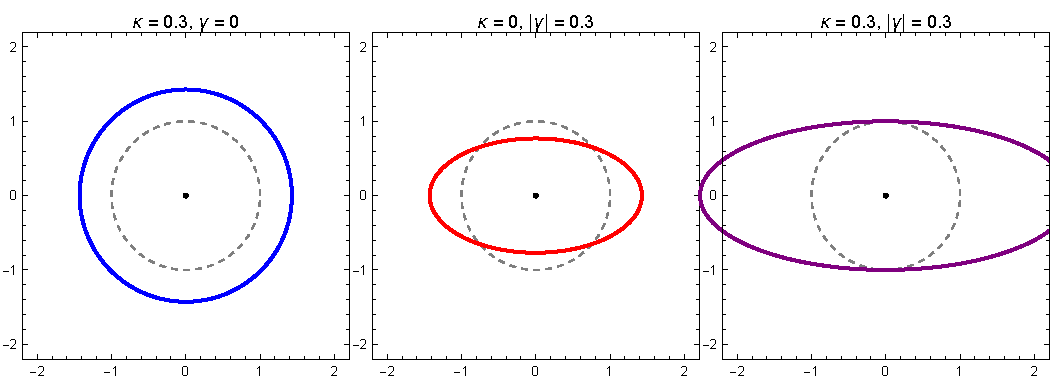
\includegraphics[width=0.85\textwidth]{../Figures/05_Magnification_Convergence_Shear/convergence_shear_effects.pdf}
    \caption{Effect of convergence and shear on a circular source.
    \textbf{Left:} Pure convergence ($\kappab = 0.3$, $\gammaL = 0$)
    produces a larger circle (isotropic magnification).
    \textbf{Center:} Pure shear ($\kappab = 0$, $|\gammaL| = 0.3$)
    produces an ellipse (anisotropic distortion; the magnification
    $\mu = 1/(1 - |\gammaL|^2) \approx 1.10$ differs from unity only at
    second order in $|\gammaL|$).
    \textbf{Right:} Both ($\kappab = 0.3$, $|\gammaL| = 0.3$) produces
    a larger ellipse.
    The dashed circle shows the original source in each panel.
    Generated by \texttt{lensing\_potential.wl}.}
    \label{fig:convergence_shear_effects}
\end{figure}


% =====================================================================
\section{Example: Point Mass Lens}
\label{sec:point_mass_example}

We now compute $\kappab$, $\gammaL$, and $\mu$ for the point mass
lens, verifying consistency with the results of
Chapter~\ref{ch:lens_equation}.

\subsection{Lensing Potential for a Point Mass}

For a point mass $M$ at the origin, the convergence is a Dirac
delta function:
\begin{equation}
    \kappab(\vectheta)
    = \frac{\Sigma(\Dd\vectheta)}{\Sigmacr}
    = \frac{M\,\delta^{(2)}(\Dd\vectheta)}{\Sigmacr}
    = \pi\thetaE^2\,\delta^{(2)}(\vectheta) \,.
    \label{eq:kappa_point_mass}
\end{equation}
The mass is concentrated entirely at the origin; away from the origin,
$\kappab = 0$.
\begin{derivation}[The factor $\pi\thetaE^2$]
A two-dimensional delta function scales as
$\delta^{(2)}(\Dd\vectheta) = \Dd^{-2}\,\delta^{(2)}(\vectheta)$, one factor of
$1/\Dd$ per dimension, because $\int\delta(ax)\,dx = 1/a$. So
$\kappab = \frac{M}{\Sigmacr\Dd^2}\,\delta^{(2)}(\vectheta)$, and
\begin{equation*}
    \frac{M}{\Sigmacr\Dd^2}
    = M\cdot\frac{4\pi\Gnewton\Dd\Dds}{\speedoflight^2\Ds}\cdot\frac{1}{\Dd^2}
    = \pi\cdot\frac{4\Gnewton M}{\speedoflight^2}\frac{\Dds}{\Dd\Ds}
    = \pi\thetaE^2 .
\end{equation*}
The total convergence $\int\kappab\,d^2\theta = \pi\thetaE^2$ is the area of
the Einstein disk: mean convergence 1 inside $\thetaE$, as for every
axisymmetric lens.
\end{derivation}

Substituting into eq.~\eqref{eq:lensing_potential}, the lensing
potential is:
\begin{equation}
    \psiL(\vectheta) = \thetaE^2 \ln|\vectheta|
    \label{eq:psi_point_mass}
\end{equation}
which satisfies $\nabla\psiL = \thetaE^2\, \vectheta/|\vectheta|^2$,
giving the deflection $\vecalpha = \thetaE^2\,\vectheta/|\vectheta|^2$
as expected.
\begin{derivation}[The convolution is trivial for a delta function]
Substituting eq.~\eqref{eq:kappa_point_mass} in eq.~\eqref{eq:lensing_potential},
$\psiL = \frac{1}{\pi}\int\pi\thetaE^2\delta^{(2)}(\vectheta')\ln|\vectheta - \vectheta'|\,d^2\theta'
= \thetaE^2\ln|\vectheta|$, by the sifting property of $\delta^{(2)}$.
\end{derivation}

\subsection{Shear for a Point Mass}

Using polar coordinates on the lens plane, we can write
$\theta_1 = \theta\cos\phi$ and $\theta_2 = \theta\sin\phi$,
where $\theta = |\vectheta|$.  Computing the second derivatives of
$\psiL = \thetaE^2 \ln\theta$:
\begin{align}
    \frac{\partial^2 \psiL}{\partial\theta_1^2}
    &= \thetaE^2\,\frac{\theta_2^2 - \theta_1^2}{\theta^4}\,, \nonumber \\[4pt]
    \frac{\partial^2 \psiL}{\partial\theta_2^2}
    &= \thetaE^2\,\frac{\theta_1^2 - \theta_2^2}{\theta^4}\,, \nonumber \\[4pt]
    \frac{\partial^2 \psiL}{\partial\theta_1\,\partial\theta_2}
    &= -\thetaE^2\,\frac{2\theta_1\theta_2}{\theta^4} \,.
    \label{eq:psi_second_derivs_point}
\end{align}
The shear components are (for $\theta \neq 0$):
\begin{align}
    \gamma_1 &= \frac{1}{2}\left(
    \frac{\partial^2\psiL}{\partial\theta_1^2}
    - \frac{\partial^2\psiL}{\partial\theta_2^2}\right)
    = -\frac{\thetaE^2(\theta_1^2 - \theta_2^2)}{\theta^4}
    = -\frac{\thetaE^2}{\theta^2}\cos 2\phi \,,
    \label{eq:gamma1_point} \\[4pt]
    \gamma_2 &= \frac{\partial^2\psiL}{\partial\theta_1\,\partial\theta_2}
    = -\frac{2\thetaE^2\,\theta_1\theta_2}{\theta^4}
    = -\frac{\thetaE^2}{\theta^2}\sin 2\phi \,.
    \label{eq:gamma2_point}
\end{align}
The shear magnitude is:
\begin{equation}
    \boxed{
    |\gammaL| = \sqrt{\gamma_1^2 + \gamma_2^2}
    = \frac{\thetaE^2}{\theta^2}
    }
    \label{eq:gamma_magnitude_point}
\end{equation}
The shear falls off as $\theta^{-2}$ and is aligned tangentially
(the factor $e^{2i\phi}$ in the complex shear).
\begin{annotation}[Why ``tangential'']
Combining eqs.~\eqref{eq:gamma1_point}--\eqref{eq:gamma2_point},
$\gammaL = -(\thetaE^2/\theta^2)e^{2i\phi} = (\thetaE^2/\theta^2)e^{2i(\phi + \pi/2)}$,
so $\phi_\gamma = \phi + 90^\circ$. The stretch axis is perpendicular to the
radius vector: the smaller eigenvalue of $\Amat$, $1 - \thetaE^2/\theta^2$, has
eigenvector $(-\sin\phi, \cos\phi)$. This is the familiar arc-like elongation
around the lens. Every axisymmetric lens has this form,
$\gammaL = -(\bar\kappab - \kappab)\,e^{2i\phi}$, and the point mass is the
case $\kappab = 0$, $\bar\kappab = \thetaE^2/\theta^2$. The overall minus
sign is why the \emph{tangential shear} is defined as
$\gammaL_{\mathrm t} \equiv -\operatorname{Re}(\gammaL e^{-2i\phi})$: it
turns this into $\gammaL_{\mathrm t} = \bar\kappab - \kappab > 0$, the form used in
Chapter~\ref{ch:axisymmetric_models} (eq.~\ref{eq:gamma_circular}) and in weak
lensing.
\end{annotation}

\subsection{Convergence for a Point Mass (away from origin)}

To compute the convergence correctly, we must be careful with the
form of $\psiL$.  Writing
$\psiL = \frac{\thetaE^2}{2}\ln(\theta_1^2 + \theta_2^2)$ in
Cartesian coordinates:
\begin{align}
    \frac{\partial\psiL}{\partial\theta_1}
    &= \frac{\thetaE^2\,\theta_1}{\theta^2} \,, \qquad
    \frac{\partial^2\psiL}{\partial\theta_1^2}
    = \thetaE^2\,\frac{\theta^2 - 2\theta_1^2}{\theta^4} \,.
\end{align}
Similarly, $\partial^2\psiL/\partial\theta_2^2
= \thetaE^2\,(\theta^2 - 2\theta_2^2)/\theta^4$.
Summing:
\begin{equation}
    \nabla^2\psiL = \thetaE^2\,
    \frac{2\theta^2 - 2(\theta_1^2 + \theta_2^2)}{\theta^4}
    = 0 \qquad (\theta \neq 0) \,.
    \label{eq:laplacian_psi_point}
\end{equation}
Therefore $\kappab = 0$ for $\theta \neq 0$, confirming that the
convergence of a point mass is indeed a delta function concentrated
entirely at the origin.  In the distributional sense,
$\nabla^2\ln|\vectheta| = 2\pi\,\delta^{(2)}(\vectheta)$, which
recovers $\kappab = \pi\thetaE^2\,\delta^{(2)}(\vectheta)$ via
the Poisson equation.

\subsection{Magnification for a Point Mass}

With $\kappab = 0$ and $|\gammaL| = \thetaE^2/\theta^2$ (for
$\theta \neq 0$), the magnification formula~\eqref{eq:magnification_formula}
gives:
\begin{equation}
    \mu = \frac{1}{1 - \thetaE^4/\theta^4}
    = \frac{\theta^4}{\theta^4 - \thetaE^4} \,.
    \label{eq:mu_point_mass}
\end{equation}
This is precisely eq.~\eqref{eq:magnification_pm} from
Chapter~\ref{ch:lens_equation}!  Evaluating at the image positions
$\theta_\pm$:
\begin{equation}
    |\mu_\pm| = \frac{u^2 + 2}{2u\sqrt{u^2 + 4}} \pm \frac{1}{2} \,,
    \qquad \mu_+ > 0 \,, \quad \mu_- < 0 \,,
    \label{eq:mu_pm_recovered}
\end{equation}
where $u = \beta/\thetaE$, recovering eq.~\eqref{eq:magnification_u}
exactly.  (The inner image has $|\theta_-| < \thetaE$, so
$\theta_-^4 - \thetaE^4 < 0$ and its signed magnification is negative.)  The consistency is verified symbolically in
\mathlink{05_Magnification_Convergence_Shear/lensing_potential.wl}{lensing\_potential.wl}.
\begin{annotation}[Reading the point mass through $\lambda_t$ and $\lambda_r$]
$\lambda_t = 1 - \thetaE^2/\theta^2$ changes sign at $\theta = \thetaE$, while
$\lambda_r = 1 + \thetaE^2/\theta^2$ never vanishes. Hence the point mass has
one critical curve, the Einstein ring. The outer image ($\theta_+ > \thetaE$)
has both eigenvalues positive (type~I). The inner one has $\lambda_t < 0 < \lambda_r$
(type~II, negative parity). There is no type~III image: it would need
$\kappab > 1 + |\gammaL|$, and the only place with $\kappab \neq 0$ is the
singular point itself.
\end{annotation}


% =====================================================================
\section{Example: Singular Isothermal Sphere (Preview)}
\label{sec:sis_preview}

The singular isothermal sphere (SIS) is the simplest realistic model
for a galaxy lens.  Its surface mass density profile is
(Congdon \& Keeton Sec.~2.3.2):
\begin{equation}
    \Sigma(\xi) = \frac{\sigma_v^2}{2\Gnewton\,\xi}
    \label{eq:sis_sigma_preview}
\end{equation}
where $\sigma_v$ is the one-dimensional velocity dispersion and
$\xi = |\vecxi|$ is the physical radius in the lens plane.

\subsection{Convergence and Shear of the SIS}

The convergence is:
\begin{equation}
    \kappab(\theta) = \frac{\Sigma(\Dd\theta)}{\Sigmacr}
    = \frac{\thetaE}{2\theta}
    \label{eq:kappa_sis}
\end{equation}
where $\thetaE = 4\pi\sigma_v^2\Dds/(\speedoflight^2\Ds)$ is the
Einstein radius of the SIS\@.  Note that $\kappab$ diverges at
$\theta = 0$ (the ``singular'' in the name) and that
$\kappab(\thetaE) = 1/2$.

The shear magnitude for the SIS is:
\begin{equation}
    |\gammaL(\theta)| = \frac{\thetaE}{2\theta}
    = \kappab(\theta) \,.
    \label{eq:gamma_sis}
\end{equation}
Remarkably, $|\gammaL| = \kappab$ at every point for the SIS\@.  This
equality does \textit{not} hold for general lens models --- it is a
special property of the isothermal profile.
\begin{derivation}[SIS convergence and shear]
\emph{Convergence.} Divide eq.~\eqref{eq:sis_sigma_preview} at $\xi = \Dd\theta$
by $\Sigmacr$:
$\kappab = \frac{\sigma_v^2}{2\Gnewton\Dd\theta}\cdot\frac{4\pi\Gnewton\Dd\Dds}{\speedoflight^2\Ds}
= \frac{2\pi\sigma_v^2\Dds}{\speedoflight^2\Ds\,\theta} = \frac{\thetaE}{2\theta}$.
\emph{Shear.} The mean convergence inside $\theta$ is
$\bar\kappab = \frac{1}{\pi\theta^2}\int_0^\theta\frac{\thetaE}{2\theta'}\,2\pi\theta'\,d\theta' = \thetaE/\theta$,
so $|\gammaL| = \bar\kappab - \kappab = \thetaE/(2\theta)$ (axisymmetric
result above). For a general power law,
$|\gammaL|/\kappab = \bar\kappab/\kappab - 1 = (\gp - 1)/(3 - \gp)$, which equals 1 only
for $\gp = 2$. This is the precise sense in which $|\gammaL| = \kappab$ is
special to the isothermal profile.
\end{derivation}

\subsection{Magnification of the SIS}

The magnification is:
\begin{equation}
    \mu = \frac{1}{(1 - \kappab)^2 - |\gammaL|^2}
    = \frac{1}{1 - 2\kappab}
    = \frac{1}{1 - \thetaE/\theta}
    = \frac{\theta}{\theta - \thetaE} \,.
    \label{eq:mu_sis}
\end{equation}
The magnification diverges at $\theta = \thetaE$ --- this is the
(tangential) critical curve of the SIS\@.  We will treat the SIS model
in full detail in Module~7.
\begin{annotation}[The SIS has no radial critical curve]
For the SIS, $\lambda_t = 1 - 2\kappab = 1 - \thetaE/\theta$ and
$\lambda_r = 1 - \kappab + |\gammaL| = 1$ exactly: all the magnification is
tangential (cf.\ Congdon \& Keeton, caption of Fig.~2.3). Note
$\kappab(\thetaE) = \tfrac12$, while the mean convergence inside $\thetaE$ is
1. A frequent slip is to locate the Einstein ring where $\kappab = 1$.
\end{annotation}


% =====================================================================
\section{Critical Curves and Caustics (Preview)}
\label{sec:critical_curves_preview}

\begin{definition}
The \textbf{critical curves} are the loci in the image plane where
the magnification diverges:
\begin{equation}
    \det \Amat(\vectheta) = 0
    \qquad \Longleftrightarrow \qquad
    (1 - \kappab)^2 = |\gammaL|^2 \,.
    \label{eq:critical_curve_condition}
\end{equation}
The \textbf{caustics} are the images of the critical curves under the
lens mapping, i.e., the corresponding curves in the source plane:
\begin{equation}
    \vecbeta_{\mathrm{caustic}} = \vectheta_{\mathrm{crit}}
    - \vecalpha(\vectheta_{\mathrm{crit}}) \,.
    \label{eq:caustic_def}
\end{equation}
\end{definition}

Critical curves and caustics play a central role in strong lensing:
\begin{itemize}
    \item When a source crosses a caustic, the number of images
          changes by two (a pair of highly magnified images appears
          or disappears).
    \item Sources near caustics are very highly magnified --- this is
          exploited in studies of distant, faint galaxies.
    \item The topology of critical curves and caustics determines the
          image configuration (doubly, quadruply, or multiply imaged
          sources).
\end{itemize}

\begin{remark}[Physical intuition for critical curves]
When $\det(\Amat) = 0$, the magnification is formally infinite.
Physically, this means that images near a critical curve are highly
stretched and magnified.  A small source near a \textit{caustic} (the
mapping of the critical curve to the source plane) produces two images
straddling the critical curve --- one with positive parity (unreflected)
and one with negative parity (mirror-reflected).  These images
appear/disappear in pairs as the source crosses a caustic, which is why
the total number of images always changes by $\pm 2$, preserving the
odd-number theorem (Module~6).  The full topological picture is
developed in Chapter~\ref{ch:elliptical_models}.
\end{remark}

For the point mass lens, the critical curve is the Einstein ring
($\theta = \thetaE$), and the caustic degenerates to a single point
($\beta = 0$).  For more complex lens models, both critical curves
and caustics have richer structures.  We will develop the full theory
in Module~8.
\begin{annotation}[Which caustic is which, for axisymmetric lenses]
A tangential critical curve ($\lambda_t = 0$, i.e.\ $\alpha(\theta) = \theta$)
maps to $\beta = \theta - \alpha = 0$: a degenerate \emph{point} caustic. For the
point mass, $\beta(\thetaE) = \thetaE - \thetaE^2/\thetaE = 0$. A radial
critical curve ($\lambda_r = 0$) maps to a \emph{circle} of radius
$|\beta(\theta_r)|$ in the source plane (Congdon \& Keeton Sec.~2.2.3).
Ellipticity or shear unfolds the point caustic into the four-cusp astroid of
Chapter~\ref{ch:elliptical_models}.
\end{annotation}


% =====================================================================
\section{Summary}
\label{sec:mag_summary}

\begin{itemize}
    \item The \textbf{lensing potential}
          $\psiL(\vectheta) = (1/\pi)\int\kappab(\vectheta')\,
          \ln|\vectheta - \vectheta'|\,d^2\theta'$ is a scalar
          field whose gradient gives the deflection angle
          ($\vecalpha = \nabla\psiL$) and whose Laplacian gives
          twice the convergence ($\nabla^2\psiL = 2\kappab$).

    \item The \textbf{convergence}
          $\kappab = \Sigma/\Sigmacr$ causes isotropic focusing:
          a circular source remains circular but changes size.

    \item The \textbf{shear} $\gammaL = \gamma_1 + i\gamma_2$
          causes anisotropic distortion: a circular source is
          stretched into an ellipse.

    \item The \textbf{Jacobian matrix}
          $\Amat = \bigl(\begin{smallmatrix}
          1-\kappab-\gamma_1 & -\gamma_2 \\
          -\gamma_2 & 1-\kappab+\gamma_1
          \end{smallmatrix}\bigr)$
          encodes all local lensing properties.  Its eigenvalues
          $\lambda_\pm = 1 - \kappab \pm |\gammaL|$ give the
          inverse magnifications along the principal axes.

    \item The \textbf{magnification}
          $\mu = 1/\det\Amat = 1/[(1-\kappab)^2 - |\gammaL|^2]$.
          The sign of $\mu$ determines the image parity.

    \item For a \textbf{point mass lens}: $\kappab = 0$ (away from
          the origin), $|\gammaL| = \thetaE^2/\theta^2$, and the
          general magnification formula recovers the result
          $|\mu_\pm| = (u^2+2)/(2u\sqrt{u^2+4}) \pm 1/2$ from Module~4,
          with $\mu_- < 0$.

    \item \textbf{Critical curves} ($\det\Amat = 0$) and their
          mappings, \textbf{caustics}, govern the image multiplicity
          and are the sites of maximum magnification.
\end{itemize}


% =====================================================================
\section{Problems}
\label{sec:mag_problems}

\begin{exercise}
\label{ex:derive_jacobian}
\textbf{(Derivation of the Jacobian matrix.)}
Starting from the lens equation $\vecbeta = \vectheta -
\vecalpha(\vectheta)$ with $\vecalpha = \nabla\psiL$:
\begin{enumerate}[label=(\alph*)]
    \item Compute $\Amat_{ij} = \partial\beta_i/\partial\theta_j$
          and express it in terms of second derivatives of $\psiL$.
    \item Decompose the Hessian matrix $\partial^2\psiL/\partial\theta_i
          \partial\theta_j$ into a trace part (proportional to
          $\delta_{ij}$) and a traceless part.  Identify the trace
          part with $\kappab$ and the traceless part with the shear.
    \item Write $\Amat$ in the form
          $\bigl(\begin{smallmatrix}
          1-\kappab-\gamma_1 & -\gamma_2 \\
          -\gamma_2 & 1-\kappab+\gamma_1
          \end{smallmatrix}\bigr)$.
\end{enumerate}
Verify with
\solnlink{05_Magnification_Convergence_Shear/problems\_05.wl}{problems\_05.wl}.
\end{exercise}

\begin{exercise}
\label{ex:poisson_2d}
\textbf{(The 2D Poisson equation.)}
\begin{enumerate}[label=(\alph*)]
    \item Show that the two-dimensional Green's function of the
          Laplacian is $(1/2\pi)\ln|\vectheta|$, i.e.,
          $\nabla^2 \ln|\vectheta| =
          2\pi\,\delta^{(2)}(\vectheta)$.
          \textit{Hint:} Use the fact that $\ln|\vectheta|$ is
          harmonic for $\vectheta \neq 0$ and apply Gauss's theorem
          to a small circle around the origin.
    \item Starting from the definition of $\psiL$
          (eq.~\ref{eq:lensing_potential}), apply the Laplacian to
          derive $\nabla^2\psiL = 2\kappab$.
    \item Verify the 2D Poisson equation for the point mass lens:
          $\psiL = \thetaE^2\ln|\vectheta|$ and
          $\kappab = \pi\thetaE^2\,\delta^{(2)}(\vectheta)$.
\end{enumerate}
Verify with
\solnlink{05_Magnification_Convergence_Shear/problems\_05.wl}{problems\_05.wl}.
\end{exercise}

\begin{exercise}
\label{ex:point_mass_shear}
\textbf{(Shear of a point mass lens.)}
For the point mass lensing potential
$\psiL = \thetaE^2\ln|\vectheta|$:
\begin{enumerate}[label=(\alph*)]
    \item Compute $\gamma_1$ and $\gamma_2$ as functions of
          $\theta_1$, $\theta_2$.
    \item Show that $|\gammaL| = \thetaE^2/\theta^2$.
    \item Express $\gamma_1$ and $\gamma_2$ in polar coordinates
          $(\theta, \phi)$ and show that the complex shear is
          $\gammaL = -(\thetaE^2/\theta^2)\,e^{2i\phi}$
          (tangential shear).
    \item Compute the ratio $|\gammaL|/\kappab$ at the image
          positions $\theta_\pm$ of the point mass lens.  What
          happens for sources far from the Einstein radius?
\end{enumerate}
Verify with
\solnlink{05_Magnification_Convergence_Shear/problems\_05.wl}{problems\_05.wl}.
\end{exercise}

\begin{exercise}
\label{ex:magnification_consistency}
\textbf{(Magnification consistency check.)}
\begin{enumerate}[label=(\alph*)]
    \item Using $\kappab = 0$ and $|\gammaL| = \thetaE^2/\theta^2$
          for the point mass lens, show that
          $\mu = \theta^4/(\theta^4 - \thetaE^4)$.
    \item Evaluate $\mu$ at the image positions $\theta_\pm =
          (\beta \pm \sqrt{\beta^2 + 4\thetaE^2})/2$.  Using
          $u = \beta/\thetaE$, show that the result reduces to
          $\mu_+ = (u^2+2)/(2u\sqrt{u^2+4}) + 1/2$ and
          $\mu_- = 1/2 - (u^2+2)/(2u\sqrt{u^2+4})$, i.e.,
          $|\mu_\pm| = (u^2+2)/(2u\sqrt{u^2+4}) \pm 1/2$.
    \item Verify that $\mu_+ > 0$ (positive parity) and
          $\mu_- < 0$ (negative parity) for all $u > 0$.
    \item Show that $|\mu_+| + |\mu_-| > 1$ for all $u > 0$
          (gravitational lensing always increases the total flux).
\end{enumerate}
Verify with
\solnlink{05_Magnification_Convergence_Shear/problems\_05.wl}{problems\_05.wl}.
\end{exercise}

\begin{exercise}
\label{ex:elliptical_image}
\textbf{(Elliptical image from constant $\kappab$ and $\gammaL$.)}
A small circular source of angular radius $\delta$ is lensed by a
region with constant convergence $\kappab$ and constant shear
$\gammaL = |\gammaL|\,e^{2i\phi_\gamma}$ (with $\gamma_1 =
|\gammaL|\cos 2\phi_\gamma$ and $\gamma_2 = |\gammaL|\sin 2\phi_\gamma$).
\begin{enumerate}[label=(\alph*)]
    \item Write the Jacobian matrix $\Amat$ for constant $\kappab$,
          $\gamma_1$, $\gamma_2$.
    \item Find the eigenvalues $\lambda_\pm$ of $\Amat$ and show
          that the image is an ellipse with semi-axes
          $a = \delta/|\lambda_-|$ and $b = \delta/|\lambda_+|$
          (assuming $|\lambda_-| < |\lambda_+|$).
    \item Compute the axis ratio $b/a$ and the magnification $\mu$
          in terms of $\kappab$ and $|\gammaL|$.
    \item The orientation of the ellipse is along the eigenvector
          corresponding to $\lambda_-$.  For $\gamma_2 = 0$
          (shear aligned with the coordinate axes), what is the
          orientation of the major axis?
    \item Evaluate the axis ratio and magnification for
          $\kappab = 0.3$, $|\gammaL| = 0.2$.
\end{enumerate}
Verify with
\solnlink{05_Magnification_Convergence_Shear/problems\_05.wl}{problems\_05.wl}.
\end{exercise}
